\documentclass[10pt,a9paper,handout]{beamer} \usepackage[utf8]{inputenc} \usepackage[francais]{babel} \usepackage[T1]{fontenc}
\usepackage{amsmath,amsfonts,amssymb,tikz,colortbl,lmodern,xspace,subfigure}
\title{Mise en place d’une expérience à très basse température et étude d’effets quantiques dans des systèmes nanométriques}
\author{Félix Piédallu}
\date{5 octobre 2015}
\institute{Grenoble INP Phelma}
\setcounter{tocdepth}{1}

\usetheme{Berlin}
\usecolortheme{beaver}
\setbeamertemplate{caption}{\raggedright\insertcaption\par}

\defbeamertemplate*{footline}{myfootline}
{
  \leavevmode%
  \hbox{%
  \begin{beamercolorbox}[wd=.32\paperwidth,ht=2.25ex,dp=1ex,left]{title in head/foot}%
    \hspace{4px}\insertshortauthor
  \end{beamercolorbox}%
  \hspace*{-5px}
  \begin{beamercolorbox}[wd=.34\paperwidth,ht=2.25ex,dp=1ex,center]{title in head/foot}%
    \insertshortinstitute
  \end{beamercolorbox}%
  \hspace*{-5px}
  \begin{beamercolorbox}[wd=.36\paperwidth,ht=2.25ex,dp=1ex,right]{title in head/foot}%
    \insertshortdate{}\hspace*{2em}
    \insertframenumber{} / \inserttotalframenumber\hspace*{2ex} 
  \end{beamercolorbox}}%
  \vskip0pt%
}
\makeatother

\setbeamertemplate{footline}[myfootline]


\newcommand{\HeT}{$^3$He\xspace}
\newcommand{\HeQ}{$^4$He\xspace}

\begin{document}
\begin{frame}
    \vspace*{-.6cm}
    \maketitle
    \begin{center}
    \vspace*{-3.3cm}
    {\footnotesize Filière PNS 2014-2015}\\[1.2cm]
    \vspace*{1.6cm}
    
\includegraphics[width=50px]{Images/logo_phelma}\qquad
    
\includegraphics[width=50px]{Images/logo_HQC}\qquad
    \hspace*{10px}
    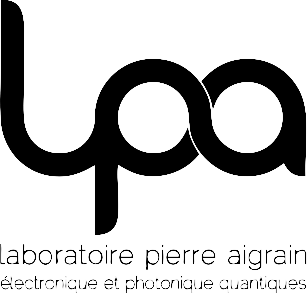
\includegraphics[width=40px]{Images/logo_lpa}\qquad
    \\[0.2cm]
    Sous la direction de Takis Kontos et Laure Bruhat
    \end{center}
\end{frame}

\begin{frame}
\tableofcontents
\end{frame}

\section*{Introduction}
\begin{frame}
    \frametitle{Introduction}
    \begin{columns}[T]
    \begin{column}{0.6\textwidth}
    {\large Hybrid Quantum Circuits} \vspace*{1mm}\\Nanotubes de carbone dans une cavité résonnante, soumis à des radiations micro-ondes
    \\[ 5mm]
    {\large Contexte du stage} \vspace*{1mm}\\
    Câblage d'une expérience dans un cryostat à dilution
    
    \end{column}
    \begin{column}{0.4\textwidth}
        \begin{figure}[H]
            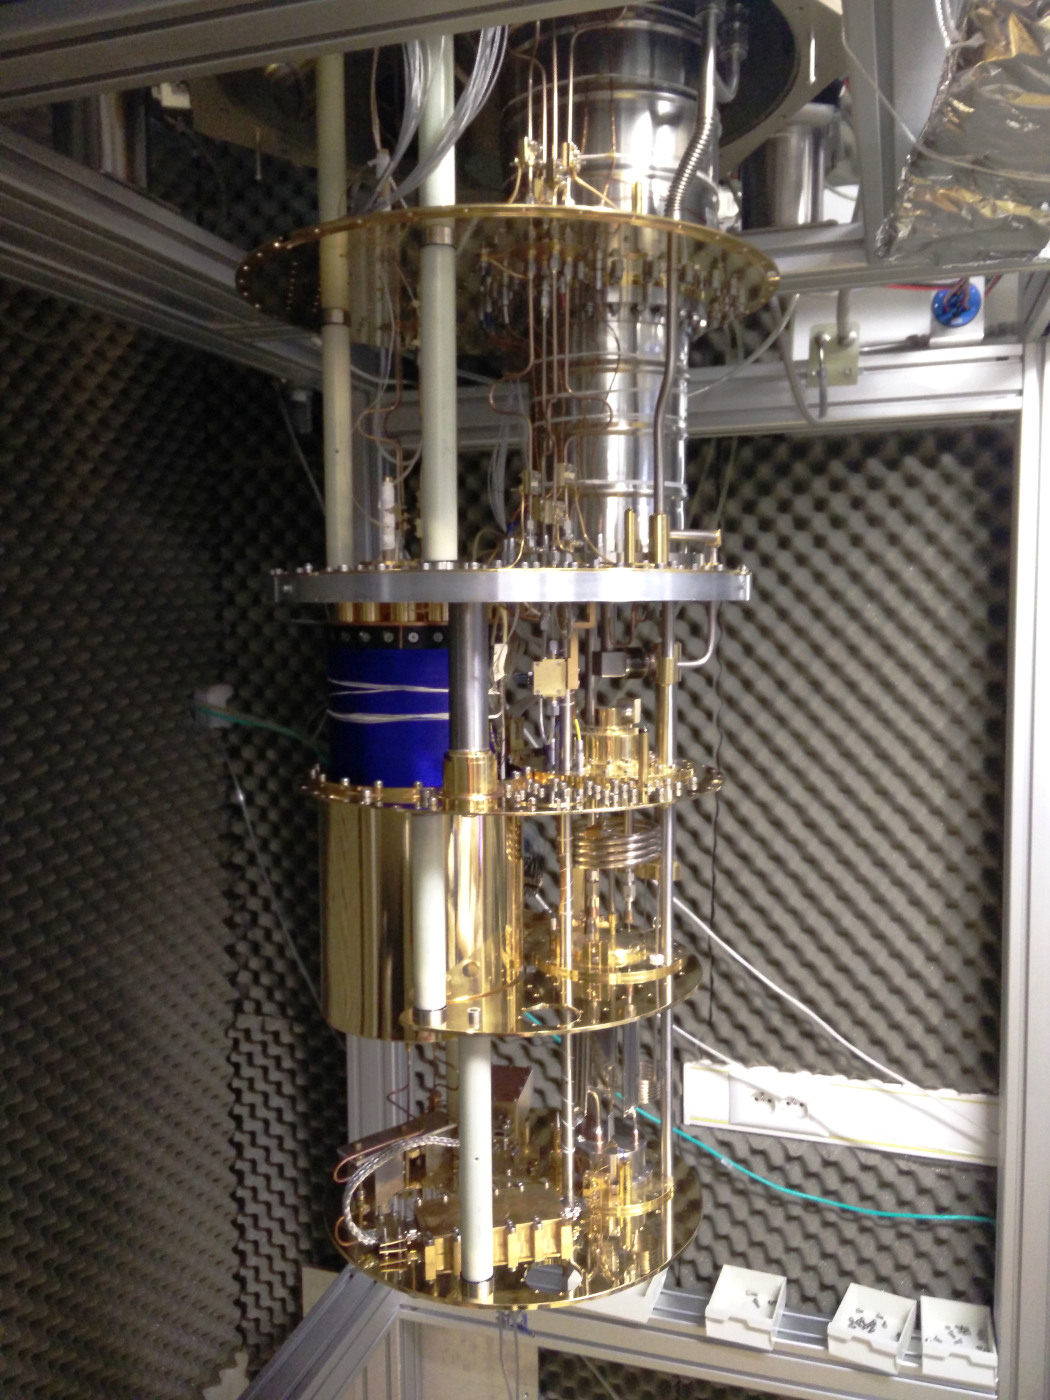
\includegraphics[width=\textwidth]{Images/Global}
            \vspace*{-3mm}\caption{Cryostat à dilution sèche}
        \end{figure}
    \end{column}
    \end{columns}
\end{frame}


\section{L'expérience}
\subsection{Injection de paires de Cooper dans un nanotube de carbone}
\begin{frame}
\begin{description}
    \item[Source :] injection de paires de Cooper intriquées
    \item[Grilles rapides :] connectées au résonateur, injection de rayonnement $\mu$Ondes
    \item[Sorties :] mesure du courant à travers chaque puits quantique 
\end{description}
\begin{figure}
    \begin{center}
        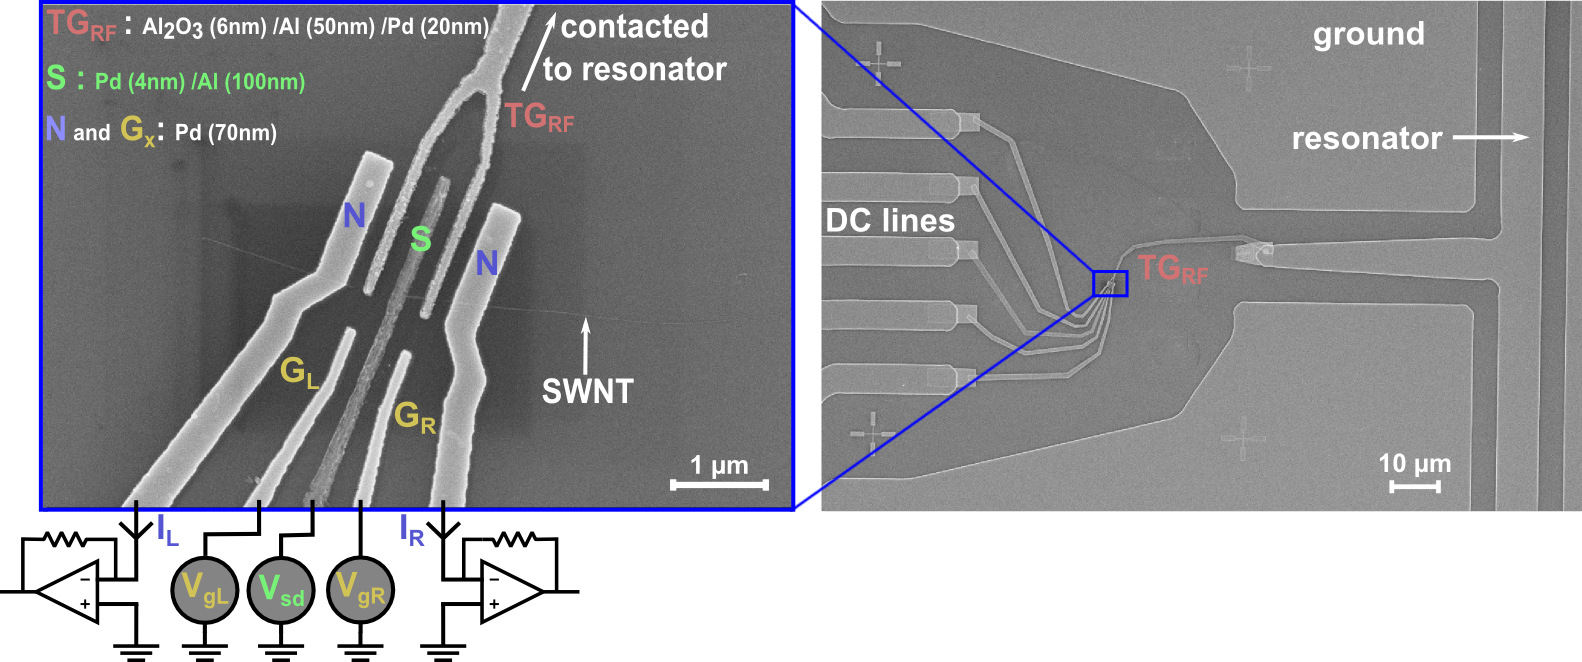
\includegraphics[width=0.6\textwidth]{Images/Expe_photo}
        \caption{Électrodes en contact avec le nanotube de carbone (SWNT)}
    \end{center}
\end{figure}
\end{frame}

\subsection{Interaction avec un rayonnement micro-ondes}
\begin{frame}
\begin{itemize}
    \item Fréquence de résonance propre de la cavité\\
        $\sim$ 6.65GHz
    \item Variation des potentiels des puits quantiques\\
    $\rightarrow$ Modification de l'impédance de la cavité\\
    $\rightarrow$ Modification des courants dans les puits quantiques
\end{itemize}

\begin{columns}[T]
\begin{column}{0.65\textwidth}
\begin{figure}[h]
    \begin{center}
        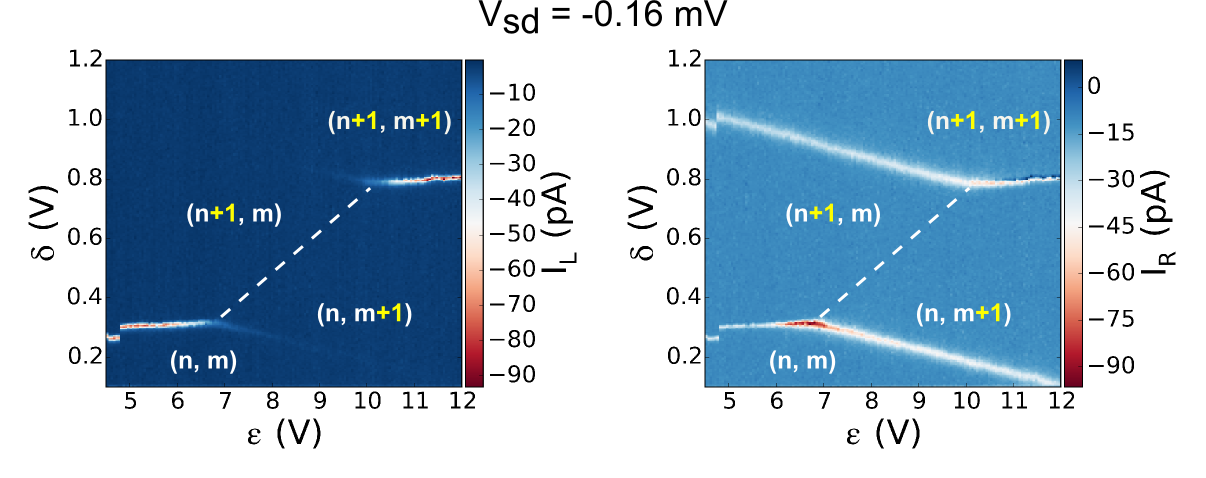
\includegraphics[width=\textwidth]{Images/Exp/CoulombBlockade}
        \caption{Blocage de Coulomb (courant dans un puits quantique)}
    \end{center}
\end{figure}
\end{column}
\begin{column}{0.35\textwidth}
\begin{figure}[h]
    \begin{center}
        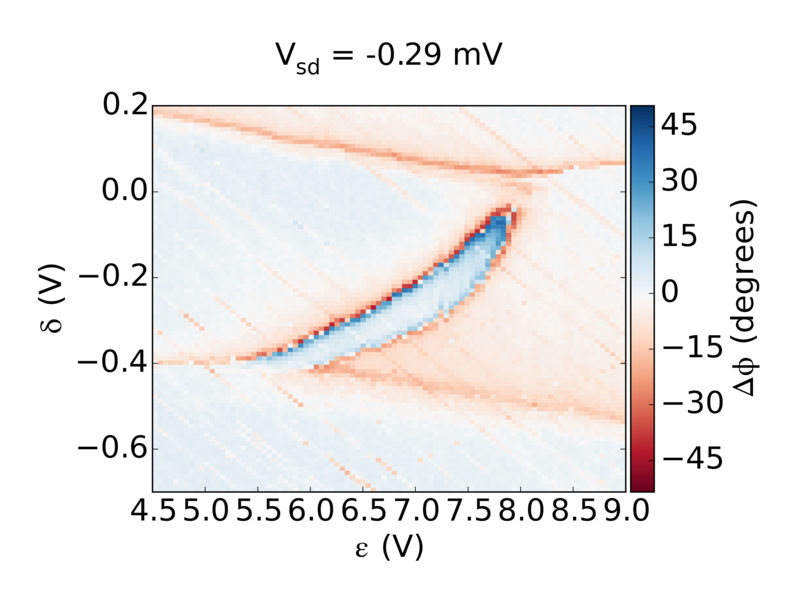
\includegraphics[width=\textwidth]{Images/Sweep/20150422_multigrayscale_DeltaEpsilon_001VsdmV_010__grayscale_phase}
        \caption{Impédance de la cavité}
    \end{center}
\end{figure}
\end{column}
\end{columns}

\end{frame}
\subsection{Nécessités de qualité d'environnement et de mesure}
\begin{frame}
\frametitle{Nécessités de qualité d'environnement et de mesure}
\begin{description}
    \item[Cohérence spatiale] ~\\
    \begin{itemize}
        \item Pas de bruit thermique
        \item Cryostat
        \item Lignes électroniques thermalisées
    \end{itemize}
    \item[Bon rapport signal/bruit] ~\\
    \begin{itemize}
        \item Choix cohérent des matériaux
    \end{itemize}
    \item[Connaissance parfaite des conditions de mesure] ~\\
    \begin{itemize}
        \item Caractérisation des câbles
    \end{itemize}
\end{description}
\end{frame}

\section{Le cryostat à dilution}
\subsection{Principe du cryostat}
\begin{frame}
\vspace*{3mm}
\begin{itemize}
    \item Extraction de l'\HeT du mélange dans le réservoir 
        ($Pp_{\: ^3\text{He}} \gg  Pp_{\: ^4\text{He}} $)
        \vspace{2mm}
    \item Réinjection de l'\HeT dans la chambre de mélange
            \vspace{2mm}
    \item Dilution de l'\HeT dans la phase diluée\\
    Réaction endothermique $\rightarrow$ Puissance calorifique
\end{itemize}

\begin{figure}[h]
  \begin{center}
    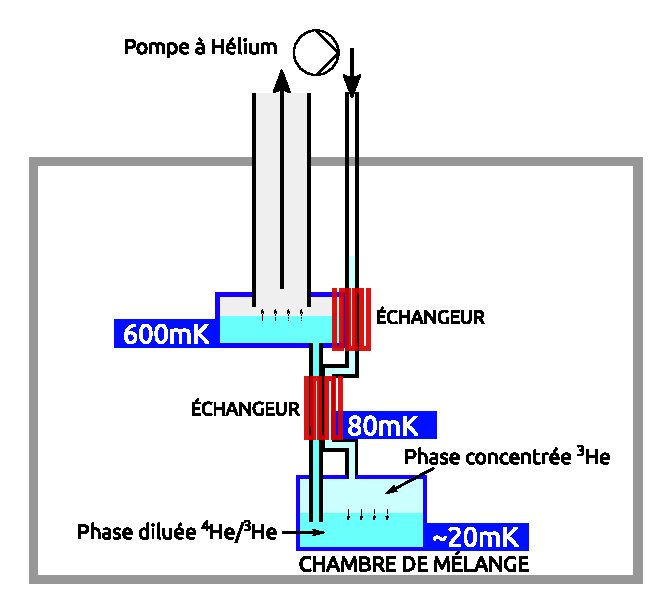
\includegraphics[width=0.42\textwidth]{Images/Cryostat_Schema.pdf}
    \qquad
    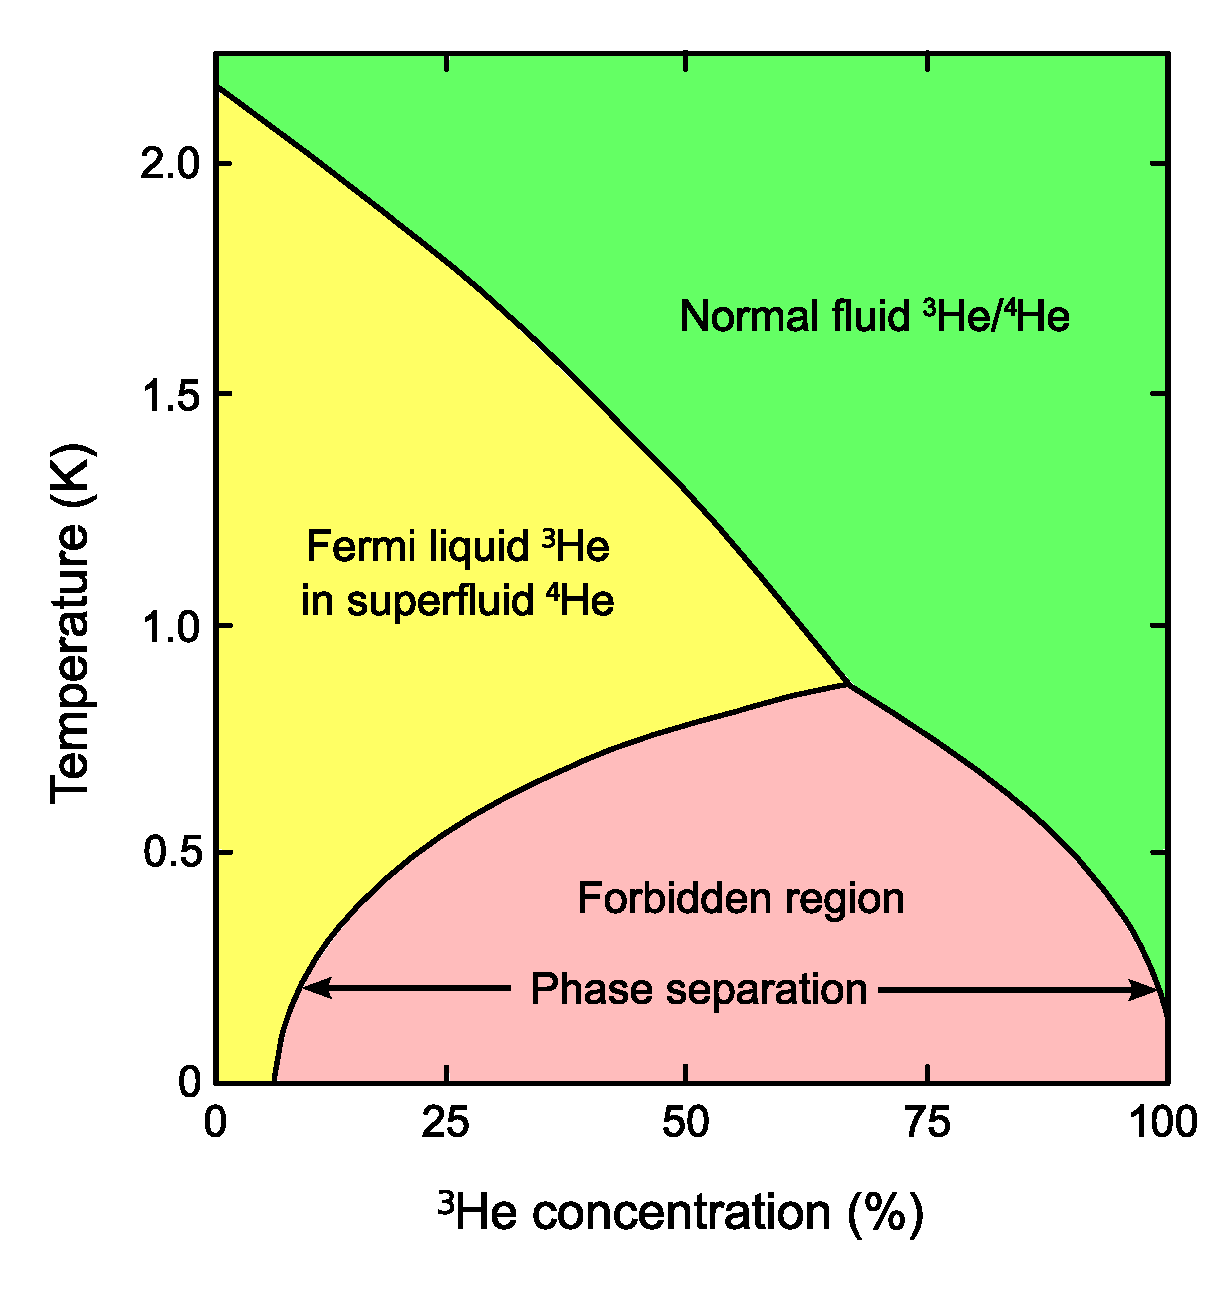
\includegraphics[width=0.23\textwidth]{Images/Helium_phase_diagram.pdf}
    \caption{Schéma du cryostat à dilution et diagramme de phase du mélange d'Hélium}
  \end{center}
\end{figure}


\end{frame}
\subsection{La dilution sèche}
\begin{frame}
\end{frame}

\section{Schéma de câblage du cryostat}
\begin{frame}
    \begin{columns}[T]
    \begin{column}{0.6\textwidth}
    \begin{itemize}
        \item Lignes Haute Fréquence
        \begin{itemize}
            \item Grilles Rapides
            \item Source (de paires de Cooper intriquées)
            \item Remontée (mesure de l'impédance de la cavité)
        \end{itemize}
        \vspace{2mm}
        \item Lignes Continues
        \begin{itemize}
            \item Potentiels des puits quantiques (Grilles)
            \item Mesures de courant
        \end{itemize}
    \end{itemize}
    \vspace{5mm}
    
    Limiter le bruit thermique des câbles \\\qquad$\rightarrow$ Résistivité élevée
    \vspace{5mm}

    Conserver un bon rapport signal/bruit \\\qquad$\rightarrow$ Atténuateurs
    
    \vspace{5mm}
    L'inverse en remontée (Peu d'atténuation)


    \end{column}
    \begin{column}{0.4\textwidth}
        \vspace*{6mm}
        \begin{figure}[H]
            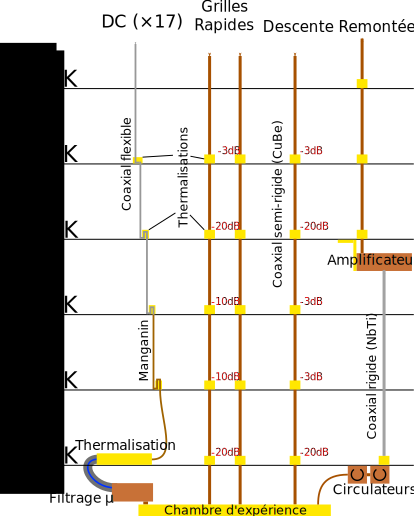
\includegraphics[width=\textwidth]{Images/Cablage_schema}
        \end{figure}
    \end{column}
    \end{columns}
\end{frame}
\section{Le câblage DC}
\subsection{Choix des matériaux}
\begin{frame}
\frametitle{Choix des matériaux}
\begin{columns}
\begin{column}{0.7\textwidth}
    \begin{description}
        \item[300K $\rightarrow$ 800mK]~\\
            Câbles coaxiaux
        \item[\hspace*{13.5mm}800mK $\rightarrow$ 20mK]~\\
            Manganin (résistif)
        \item[\hspace*{28.5mm} 20mK $\rightarrow$ porte-échantillons]~\\
            Câbles peu résistifs
    \end{description}
\end{column}
\begin{column}{0.3\textwidth}
\begin{figure}[h]
    \begin{center}
        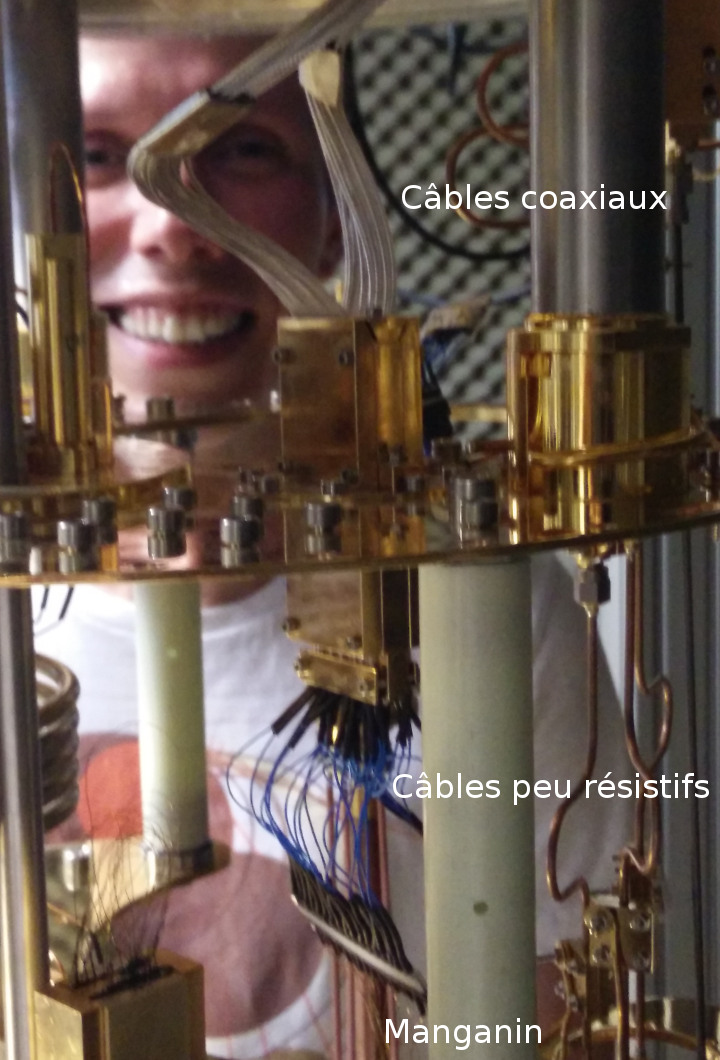
\includegraphics[width=\textwidth]{Images/Thermalisation/Etage_Tuteur}
        \caption{Aperçu des câbles DC}
    \end{center}
\end{figure}
\end{column}
\end{columns}

\end{frame}
\subsection{Thermalisation électronique}
\begin{frame}
\frametitle{Thermalisation à chaque étage}

\begin{columns}
\begin{column}{0.6\textwidth}
    \begin{itemize}
        \item Diminuer le bruit électronique au fur et à mesure
        \vspace*{5mm}
        \item Presses dorées à chaque étage \\
        + Stycast (époxy cryogénique)
        \vspace*{5mm}
        \item Câbles résistifs pour isolation thermique
    \end{itemize}
\end{column}
\begin{column}{0.3\textwidth}
\begin{figure}
    \begin{center}
        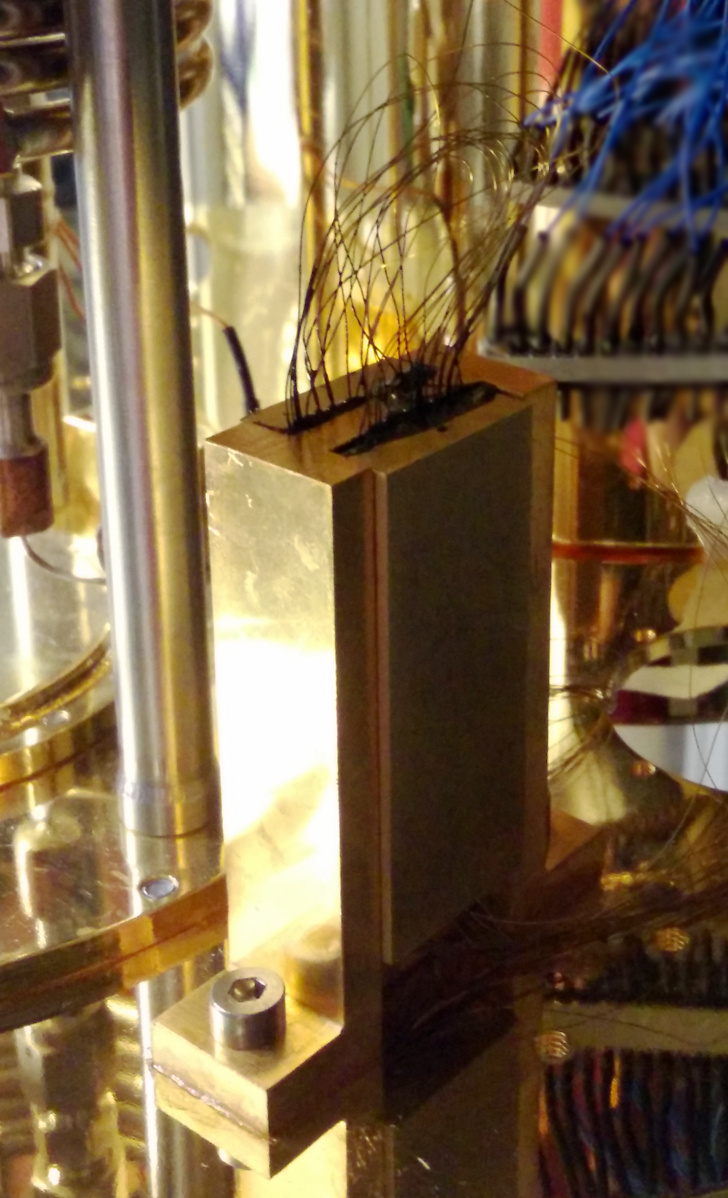
\includegraphics[width=\textwidth]{Images/Thermalisation/DC}
        \caption{Fils de Manganin "stycastés"}
    \end{center}
\end{figure}
\end{column}
\end{columns}
\end{frame}

\begin{frame}
\frametitle{Boîtier de thermalisation électronique}
\begin{columns}
\begin{column}{0.6\textwidth}
    \begin{itemize}
        \item Dernière thermalisation à 20mK (Méandres)
        \vspace*{2mm}
        \item Filtre passe-bas (premier filtrage)
    \end{itemize}
\end{column}
\begin{column}{0.3\textwidth}
\begin{figure}[h]
    \begin{center}
        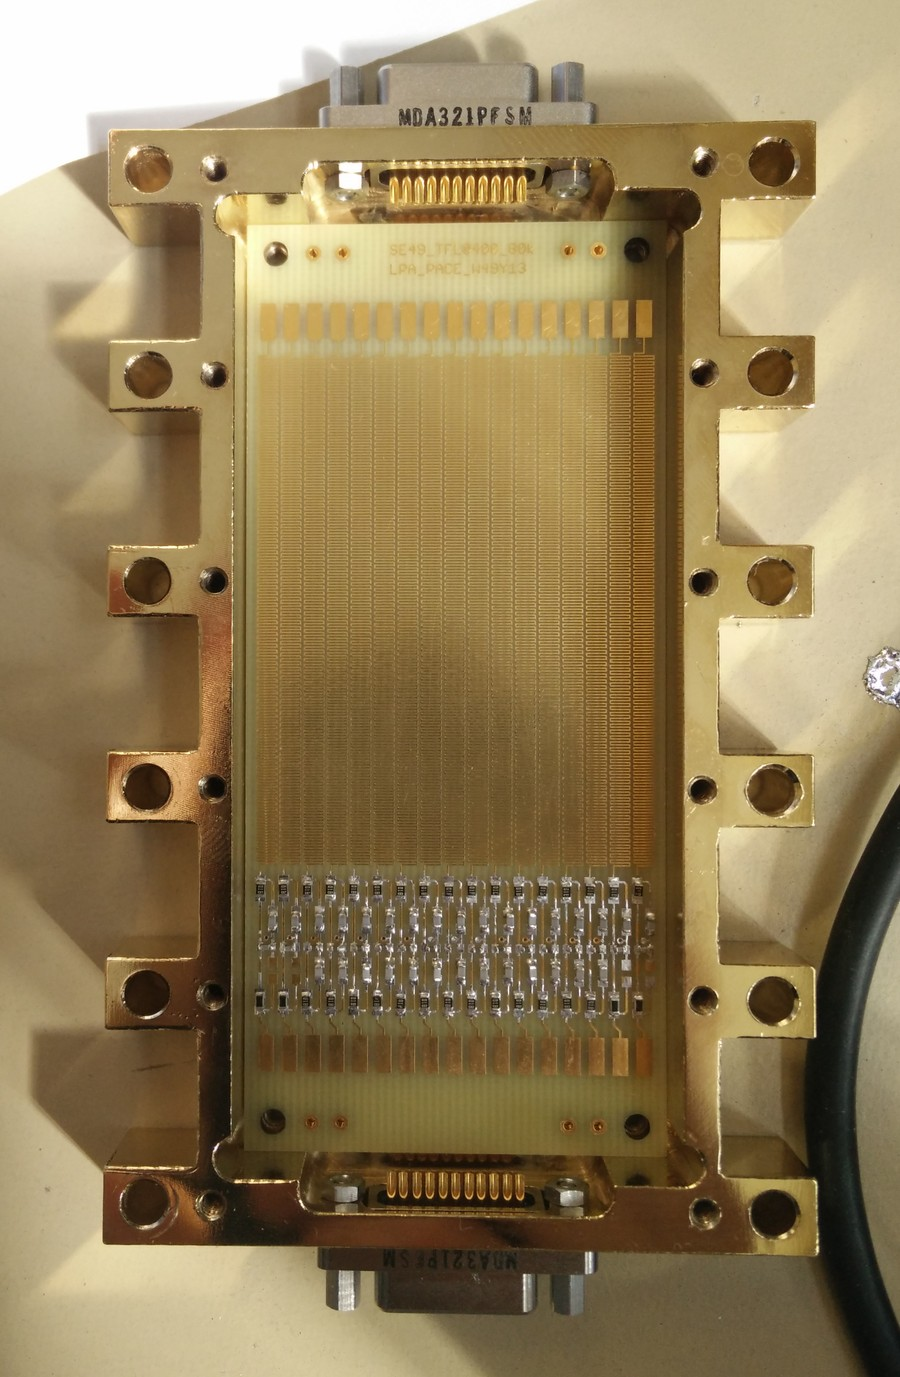
\includegraphics[width=\textwidth]{Images/Thermalisation/DC3_non_rotate}
        \caption{Boîtier non soudé}
    \end{center}
\end{figure}
\end{column}
\end{columns}

\end{frame}

\begin{frame}
\frametitle{Boîtier de filtrage micro-ondes}

\begin{itemize}
    \item Filtrage micro-ondes grâce à l'Eccosorb
    \vspace*{2mm}
    \item Compartimentage du boîtier\\
    \hspace*{1cm} $\rightarrow$ Impression 3D de prises
\end{itemize}
\vspace*{3mm}
\begin{figure}[h]
    \centering
    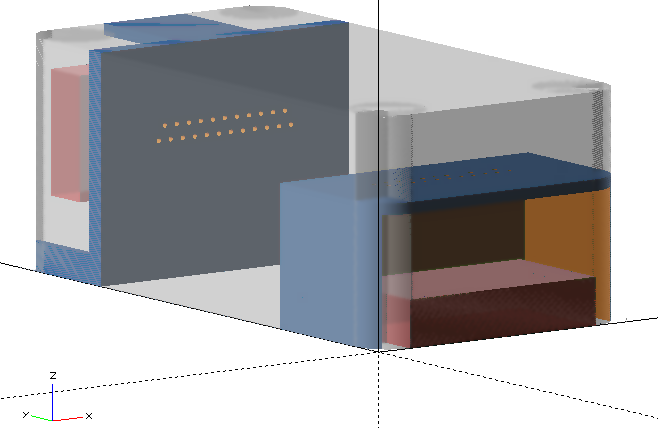
\includegraphics[height=0.25\textwidth]{Images/Thermalisation/Filtrage3D}
    ~ 
    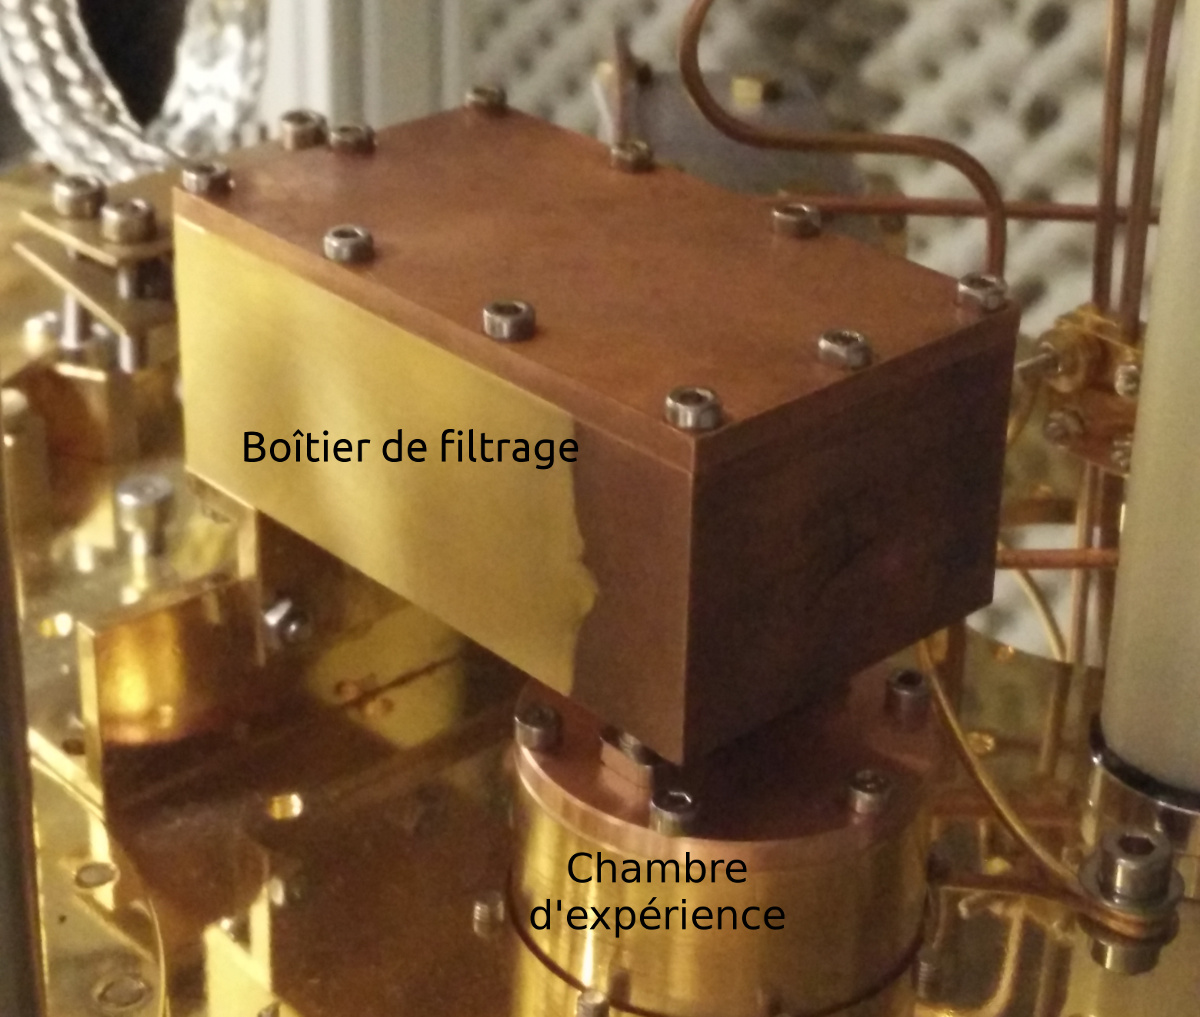
\includegraphics[height=0.25\textwidth]{Images/Thermalisation/Filtrage}
    \caption{Boîtier modélisé, puis une fois installé}
\end{figure}
\end{frame}

\subsection{Blindage des câbles}

\begin{frame}
\begin{itemize}
    \item Protection au rayonnement des étages supérieurs
    \vspace*{2mm}
    \item Protection au champ magnétique\\
\end{itemize}

\vspace*{3mm}
\begin{figure}[h]
    \centering
    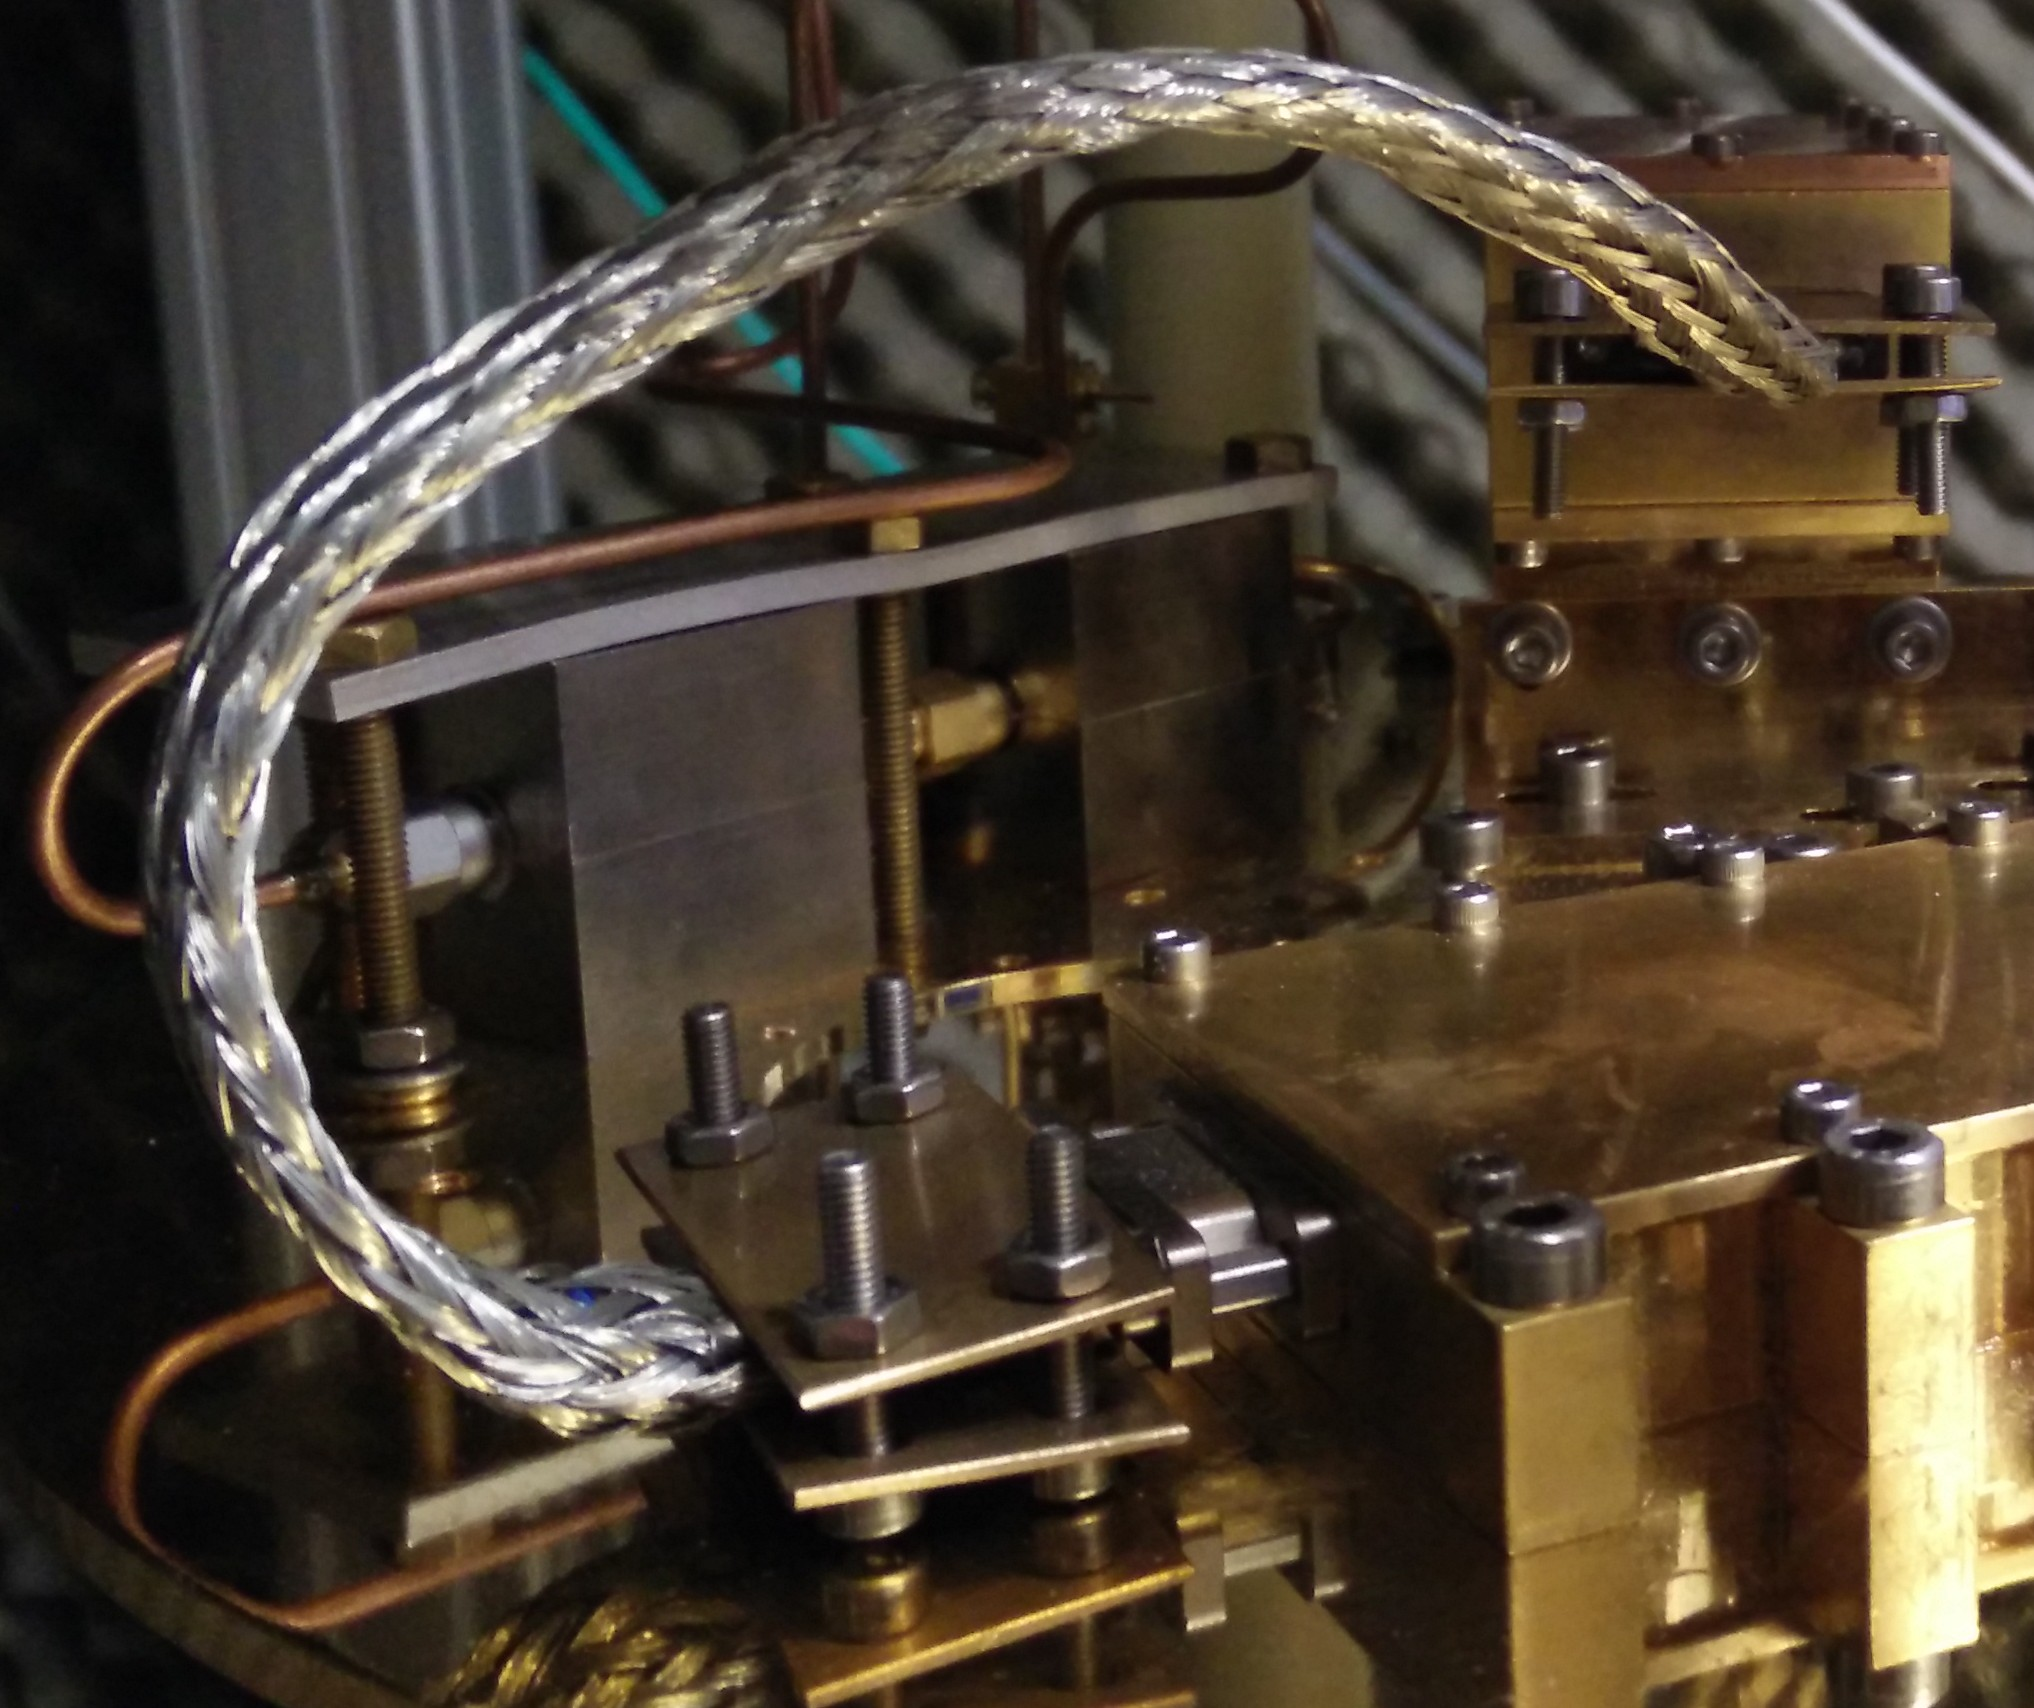
\includegraphics[height=0.35\textwidth]{Images/Tresse}
    \caption{Tresse connectée aux boîtiers de thermalisation et de filtrage}
\end{figure}
\end{frame}

\section{Le câblage RF}
\subsection{Choix des matériaux}
\begin{frame}
\begin{columns}
\begin{column}{0.7\textwidth}
    \begin{description}
        \item[Descente jusqu'à 20mK]~\\
            Cuivre-Béryllium (impédance élevée)
        \item[Étage 20mK]~\\
            Cuivre (faible impédance)
        \item[Remontée à 4K]~\\
            Niobium-Titane \\(très faible impédance)
        \item[Remontée (après ampli à 4K)]~\\
            Cuivre-Béryllium
    \end{description}
\end{column}
\begin{column}{0.3\textwidth}
\begin{figure}[h]
    \begin{center}
        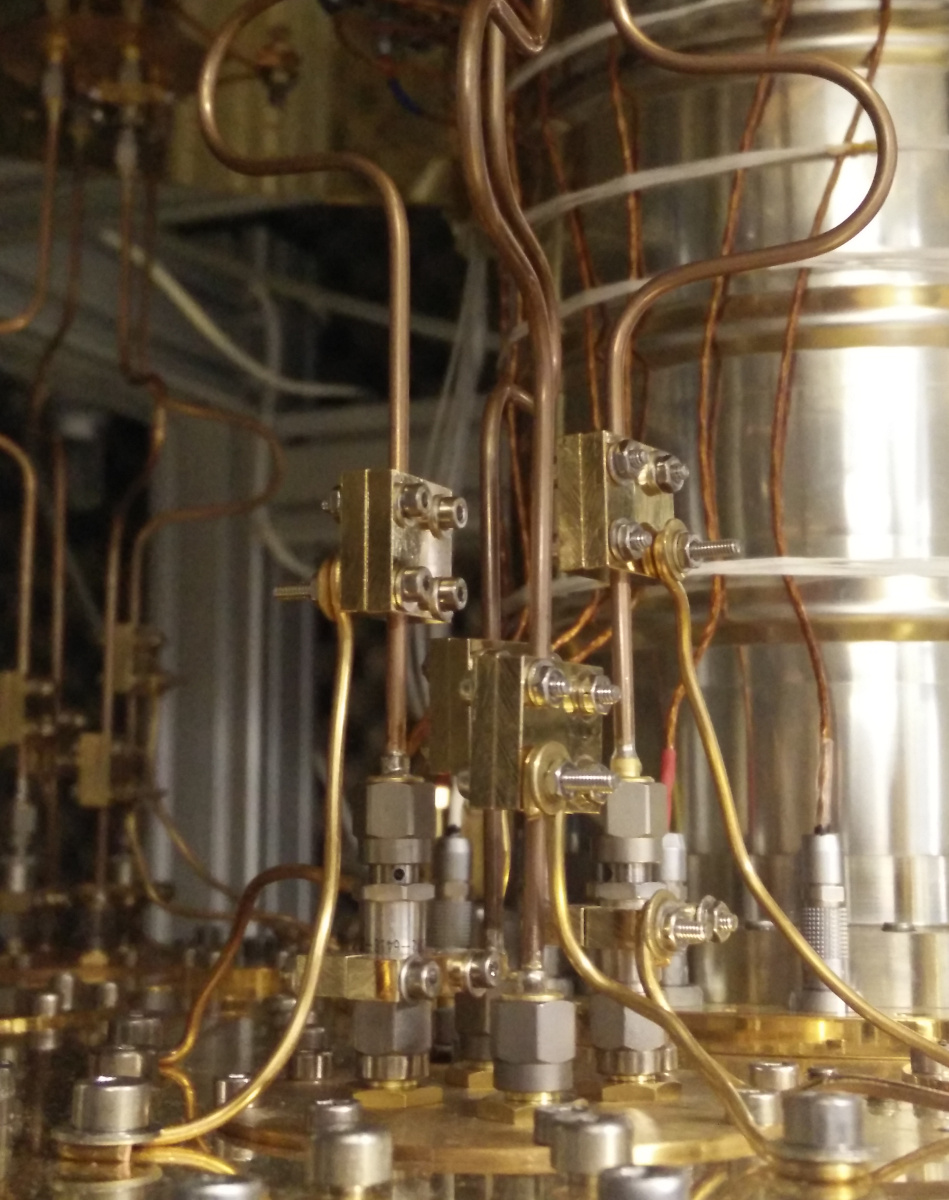
\includegraphics[width=\textwidth]{Images/Coax}
        \caption{Les différents câbles coaxiaux}
    \end{center}
\end{figure}
\end{column}
\end{columns}
\end{frame}

\subsection{Fabrication d'un câble coaxial}
\begin{frame}
\frametitle{Dénudage et soudure de la pin centrale}
\begin{columns}
\begin{column}{0.5\textwidth}
\begin{figure}[h]
    \begin{center}
        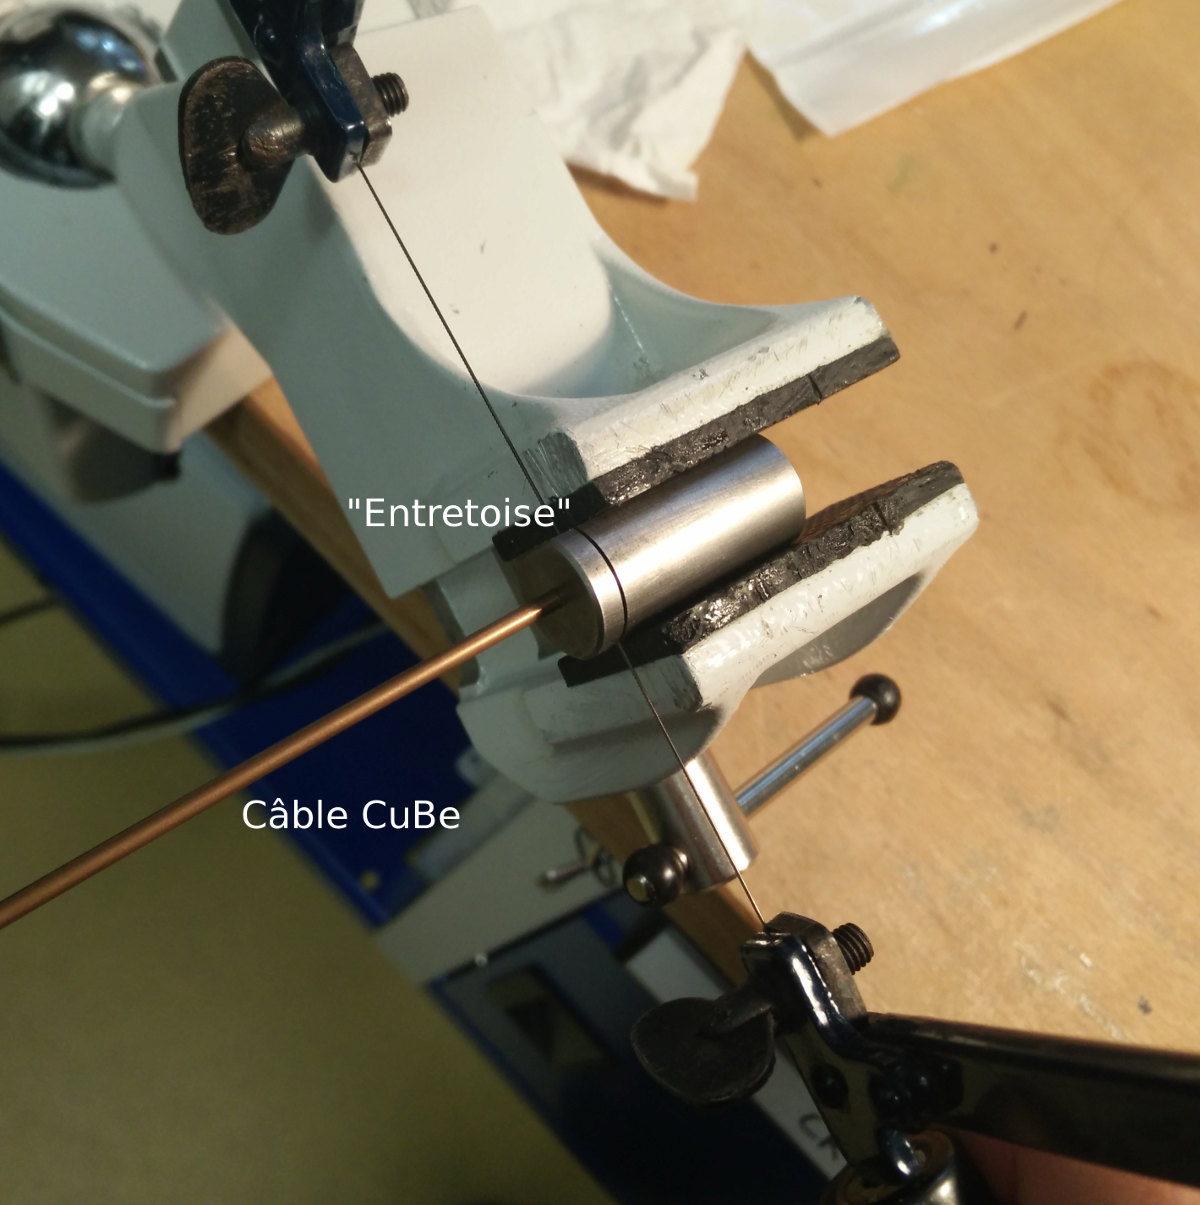
\includegraphics[width=\textwidth]{Images/Coax/1}
        \caption{Dénudage d'un câble coaxial}
    \end{center}
\end{figure}
\end{column}
\begin{column}{0.5\textwidth}
\begin{figure}[h]
    \begin{center}
        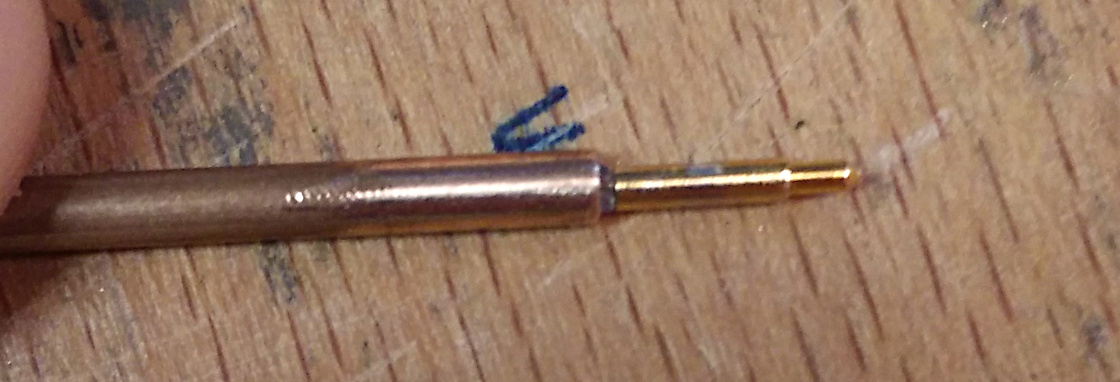
\includegraphics[width=\textwidth]{Images/Coax/3}
        \caption{Pin centrale soudée}
    \end{center}
\end{figure}
\end{column}
\end{columns}
\end{frame}

\begin{frame}
\frametitle{Prise extérieure et diélectrique}
\begin{columns}

\begin{column}{0.5\textwidth}
\begin{figure}[h]
    \begin{center}
        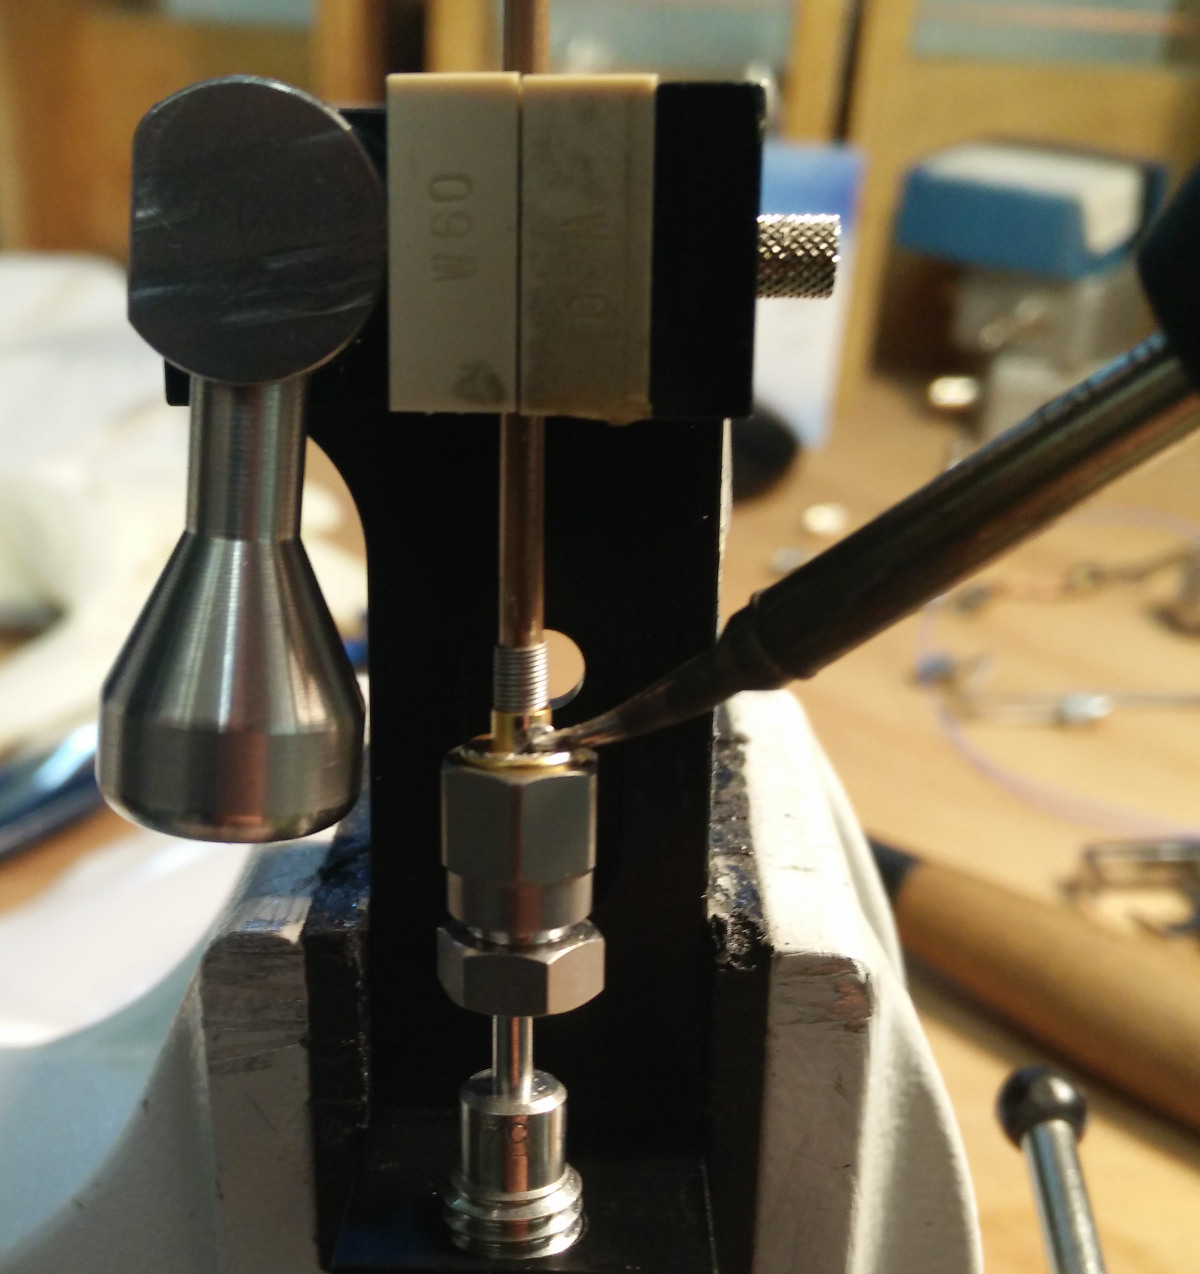
\includegraphics[width=\textwidth]{Images/Coax/4}
        \caption{Soudure de la prise extérieure}
    \end{center}
\end{figure}
\end{column}
\begin{column}{0.5\textwidth}
\begin{figure}[h]
    \begin{center}
        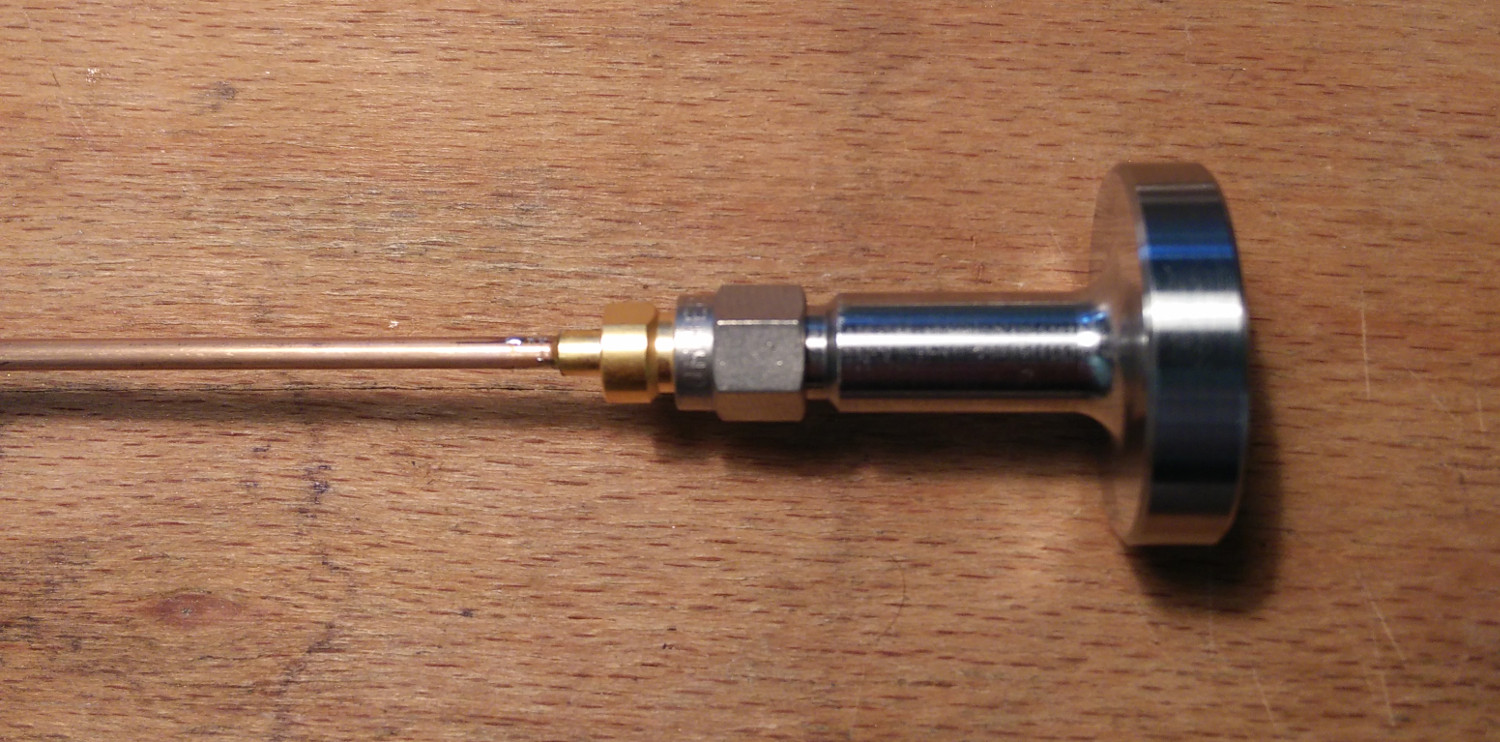
\includegraphics[width=\textwidth]{Images/Coax/6}
        \caption{Emboutissage du diélectrique}
    \end{center}
\end{figure}
\end{column}
\end{columns}
\end{frame}


\begin{frame}
\frametitle{Cintrage du câble}
\begin{columns}
\begin{column}{0.5\textwidth}
    \begin{description}
        \item[]~\\
    \end{description}
\end{column}
\begin{column}{0.5\textwidth}
\begin{figure}[h]
    \begin{center}
        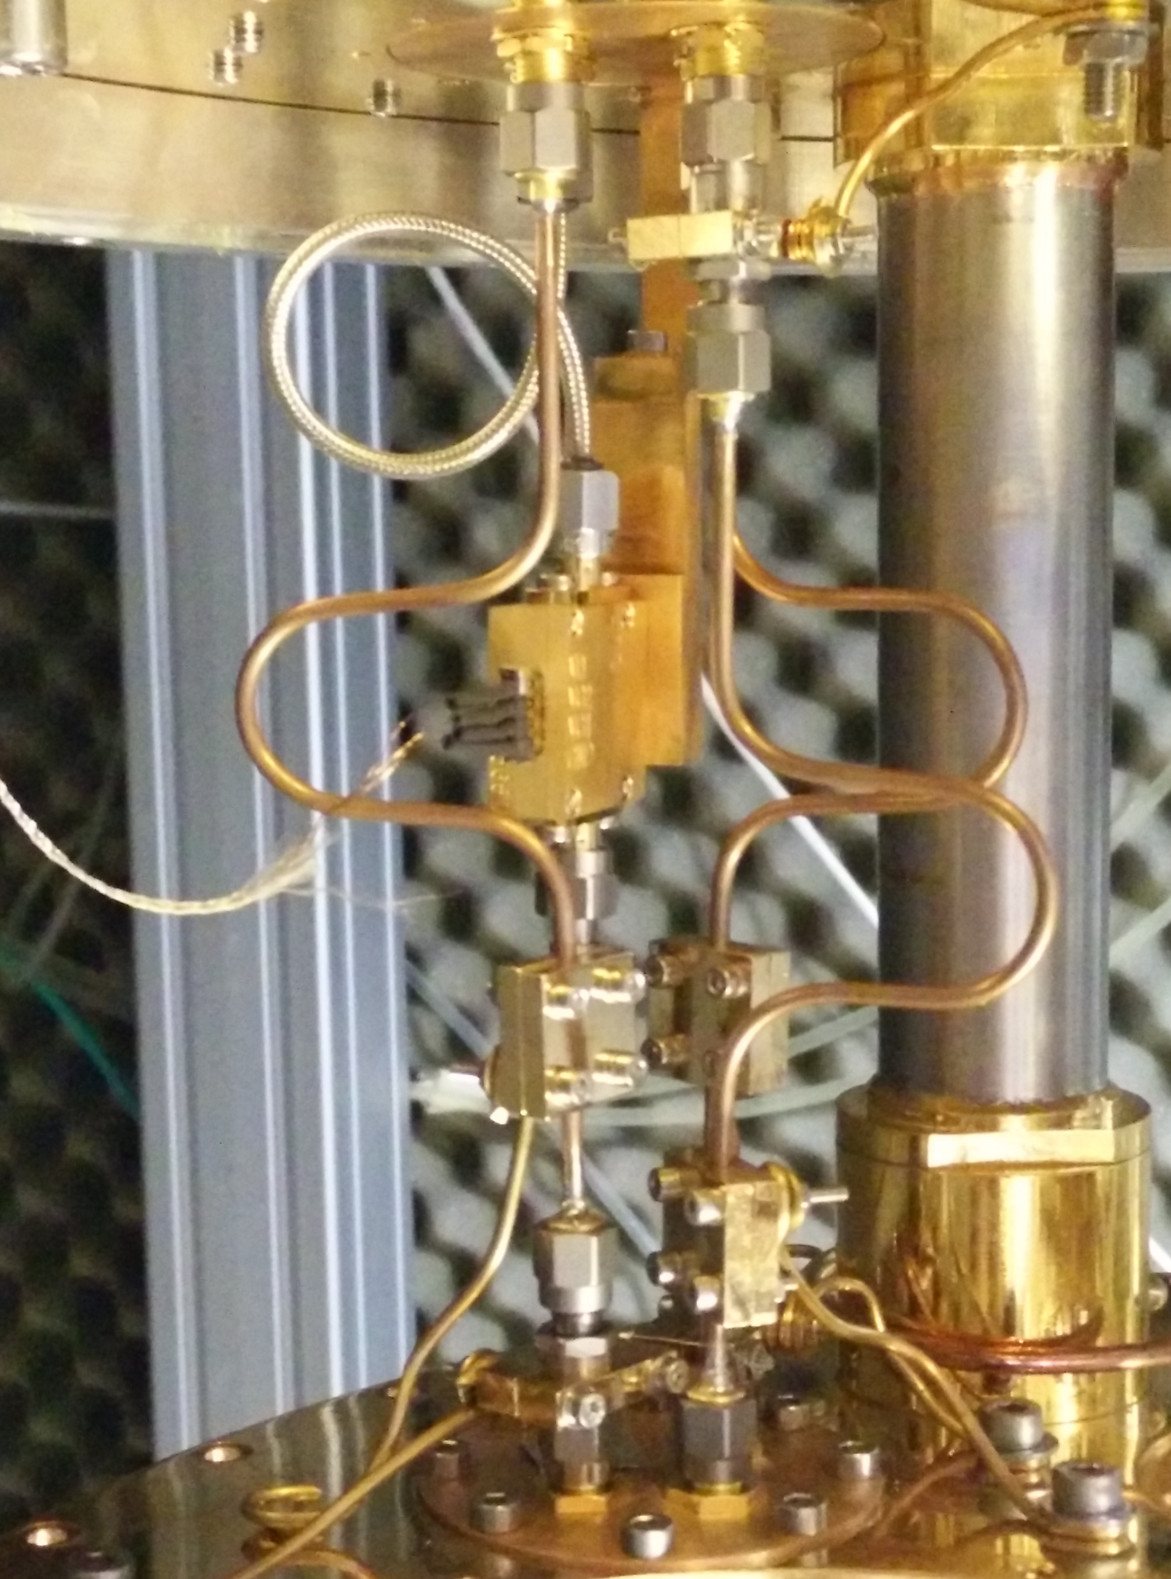
\includegraphics[width=0.7\textwidth]{Images/Coax/cintrage}
        \caption{Câbles coaxiaux cintrés en place}
    \end{center}
\end{figure}
\end{column}
\end{columns}
\end{frame}

\section{Caractérisation des câbles coaxiaux}
\subsection{Utilisation du PNA}
\begin{frame}
\frametitle{Le Performance Network Analyzer \tiny{ ou Vector…} }
\begin{columns}
\begin{column}{0.6\textwidth}
    \begin{description}
        \item[]~\\
    \end{description}
\end{column}
\begin{column}{0.4\textwidth}
\begin{figure}[h]
    \begin{center}
        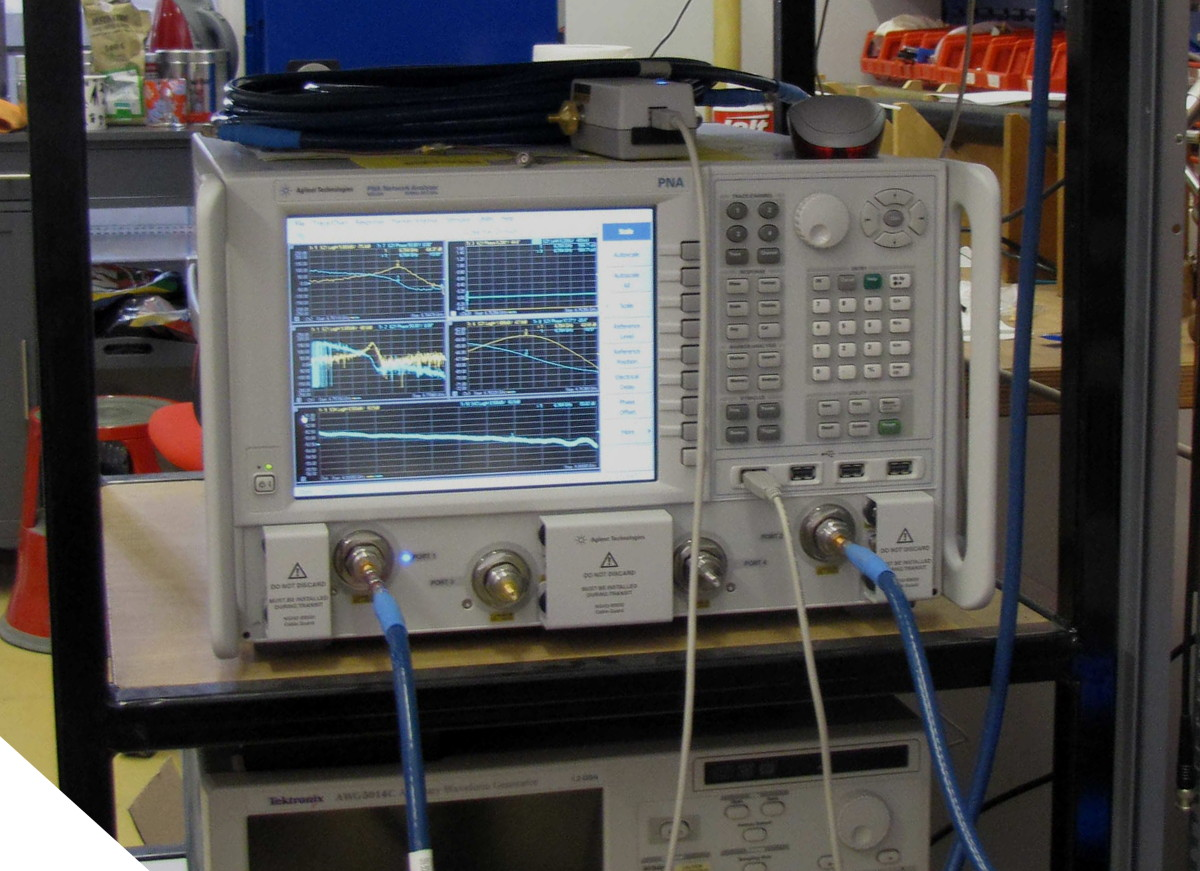
\includegraphics[width=\textwidth]{Images/VNA}
        \caption{Le PNA de l’équipe}
    \end{center}
\end{figure}
\end{column}
\end{columns}
\end{frame}



\begin{frame}
    \begin{LARGE}
    \begin{center}
    \textbf{Merci de votre attention !}
    \vspace{0.5cm}
    
    \textbf{Place aux questions.}
    \end{center}
    \end{LARGE}
\end{frame}
\end{document}
